% TEMPLATE for Usenix papers, specifically to meet requirements of
%  USENIX '05
% originally a template for producing IEEE-format articles using LaTeX.
%   written by Matthew Ward, CS Department, Worcester Polytechnic Institute.
% adapted by David Beazley for his excellent SWIG paper in Proceedings,
%   Tcl 96
% turned into a smartass generic template by De Clarke, with thanks to
%   both the above pioneers
% use at your own risk.  Complaints to /dev/null.
% make it two column with no page numbering, default is 10 point

% Munged by Fred Douglis <douglis@research.att.com> 10/97 to separate
% the .sty file from the LaTeX source template, so that people can
% more easily include the .sty file into an existing document.  Also
% changed to more closely follow the style guidelines as represented
% by the Word sample file. 

% Note that since 2010, USENIX does not require endnotes. If you want
% foot of page notes, don't include the endnotes package in the 
% usepackage command, below.

% This version uses the latex2e styles, not the very ancient 2.09 stuff.
\documentclass[letterpaper,twocolumn,10pt]{article}
\usepackage{usenix,epsfig,endnotes,graphicx}
\usepackage{epstopdf, color}
\usepackage{enumitem}
\setlist[enumerate]{itemsep=0mm}
% \DeclareGraphicsExtensions{.eps}

\begin{document}

%don't want date printed
\date{}

%make title bold and 14 pt font (Latex default is non-bold, 16 pt)

\title{\Large \bf BugBox : A Vulnerability Corpus for PHP Web Applications}


%for single author (just remove % characters)
\author{
{\rm Gary Nilson}\\
Computer Science Department\\University of Maryland
\and
{\rm Kent Wills}\\
Computer Science Department\\University of Maryland
\and
{\rm Jeff Stuckman}\\
Computer Science Department\\University of Maryland
\and
{\rm Jim Purtilo}\\
Computer Science Department\\University of Maryland
% copy the following lines to add more authors
% \and
% {\rm Name}\\
%Name Institution
} % end author

\maketitle

% Use the following at camera-ready time to suppress page numbers.
% Comment it out when you first submit the paper for review.
\thispagestyle{empty}

\subsection*{Abstract}

Web Applications provide a robust amount of code vulnerabilities that are exploited on a routine basis, but a large, diverse, automated, ease of use corpus for analyzing these vulnerabilities is not publicly available.   BugBox, an open-source corpus and framework for PHP web application vulnerabilities was created to fill this void and in doing so encourage community support to enhance the quality of the project.  We discuss the easy to use framework for web applications and further explain the motivation behind and application of BugBox.  Through our framework implementation and corpus we can enhance testing vulnerability indicators and metrics, developing vulnerability definition representations, testing intrusion detection systems, or creating demonstrations for training purposes.  

\section{Introduction}
Web applications are subject to a rich variety of exploit types, such as cross-site scripting (XSS), cross-site request forgery (XSRF), buffer overflow, and SQL injection.  Many of these web applications are designed in PHP, for which Top Cyber Security Risks has reported to be a target for security threats [ref].  This variety and preponderance of exploits is logged extensively in popular exploit databases such as the National Vulnerability Database (NVD), Open Source Vulnerability Database (OSVDB), Common Vulnerability and Exposures Database (CVE), or the Exploit Database (EDB).\\

While many of these databases exist and disclose the details of the vulnerability and/or exploit, many do not provide a collection of structured vulnerable code that can be used for analysis.  A suitable, structured collection of vulnerable code is typically not made publicly available and is scarce in quantity.  The structured collection, often reffered to as a corpus, is useful in statistical analysis and hypothesis testing if it meets certain criteria.  To elaborate on the suitability of a corpus, one most consider several of these criteria, which include: representativeness of the samples, quantity of the samples, diversity of the samples, and reproducability of the tests that produced the samples.  \\

Uses of a corpus of this type include: serving as a training aid for security teams, penetration testing, testing static analysis tools, and metric based analysis.  Projects such as ``An empirical investigation into open source web applications' implementation vulnerabilities" by Huynh and Miller\cite{DBLP:journals/ese/HuynhM10} could have benefitted from a corpus of this type. Insert our projects here.\\

Understanding the scarcity and labor involved in developing a corpus that is suitable, has led to the in-house creation of BugBox, a publicly available, scalable, efficient, easy-to-use framework and corpus that collects vulnerable code signatures through an automated trace based collection method.  To increase the sample size and diversity of BugBox, we must attract community support.  In order to successfully use this support, we provide a framework that is easy to maintain, quick to use, automated, fully compartmentalized, and scalable.  Through the use of abstraction and encapsulation, the management of application, environment, and exploitation has been streamlined in BugBox.  The design is intended to make it practical to manage a large database of exploits, along with their target environments. Our corpus is more than an exploit repository, it contains the software and its dependencies in which a vulnerability exists, the configuration of the software in it's vulnerable state, exploit code that will trigger the security breach, and data that describes any distinguishing attributes of the bug. [define attributes futher]\\

evaluating static analysis tools\cite{Zitser:2004:TSA:1041685.1029911}, penetration testing and training security teams with vulnerablity injection\cite{4725309}, and computing attack surface metrics.\cite{Stuckman:2012:CAA:2372225.2372229}\\

\section{Vulnerability Representation}

A few effective methods for finding which piece of code creates a vulnerable condition in a program are line-based, run-based, and trace-based approaches.  Henceforth, we will refer to these  methods as \emph{vulnerability localization}.  Works by Fonseca and Vieira\cite{4630094} use a line-based approach for vulnerability collection.  This approach uses line numbers represented in program patches to identify the location of the vulnerabilities.  Whil, in general, this is a sound approach, patches in a program may only mask the vulnerable code instead of replace it.  Other by Song\cite{Song:2008:BNA:1496255.1496257} create vulnerability signatures from intermediate byte code.  This approach, while quick and efficient cannot be used for a PHP web application.  The method proposed for our corpus is a trace-based collection approach in order to capture code vulnerabilities in software.  The trace-based collection method is performed through monitoring the programs execution through the use of XDebug.

\section{Requirements}

BugBox is designed to work with the Debian GNU/Linux distribution and compatible distributions.  It can be distributed as a self-contained virtual machine, or as a package that can be installed on an existing system. The machine must have sufficient storage (roughly 4 GB per OS environment, and 2 GB for the application, engine, and exploit sources [Confirm these \#s]).  Dependencies for BugBox include MySQL,  Selenium Server, debootstrap, and the Advanced Packaging Tool (APT.)\par

\section{Environment}

In order to conduct tests in an isolated environment we use a virtual jail, the linux chroot environment.  Staging the application in the chroot environment provides locality, reproducibility, and stability and flexibility.\\

{\bf The web application remains local}.  Many applications, such as wordpress, have a MYSQL backend.  If we were to host the application on a different server or VM we would have to ensure that the MYSQL database is properly setup each time.  With the chroot environment, the process is simplified, we keep a MYSQL database outside of the CHROOT Jail in order to facilitate MYSQL access.  \\

{\bf Current tests are independent from future tests}.  We load a clean application into the chroot jail every time we wish to run a new test.  This ensures that there is no corruption of the original web application and provides reproducible results when testing.\\

{\bf The web application cannot contaminate our testing environment}.  If a web application crashes due to the malicious script, we can ensure that it does not crash our corpus environment.  In the worst case the chroot becomes corrupt for which we can treat in an isolated scenario tha does not have un-intended side effects in our testing environment.  \\

{\bf The web application will never be contaminated}.  We store a separate backup in order to verify that the selenium scripts did not modify the Web Application in any way.  If the Web Application is corrupt, then we simply copy the web application from the backup folder to the package folder.  Future implementations will store only the md5 hash of the program on the corpus server and the backups on an external server.  This will allow for a quick comparison followed by a remote copy for mismatched hashes.  This separation will ensure that backups will never be corrupted through use of the corpus and expedite checking.  \\

{\bf Applications with different OS environments can be run}.  If an application was built for debian 6 as opposed to debian 4, we can setup a chroot environment that has support for that specific OS.  This gives us the flexibility to test the web application in whatever OS environment we choose.\\

\section{Framework}

\begin{figure}[!tp]
\begin{center}
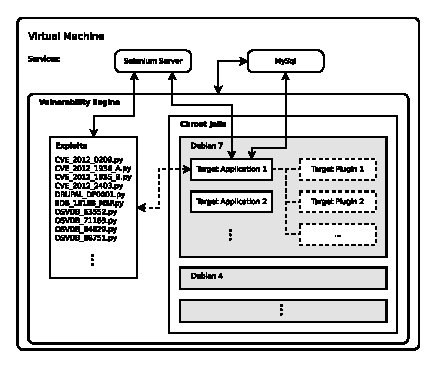
\includegraphics[scale=1.17]{system_diagram.eps}
\end{center}
\caption{System Diagram}
\end{figure}

At the the core components of the BugBox framework are driven by the Python module and package system. The system breaks down into the following four python modules: corpus.{\bf Engine}, corpus.{\bf Targets}, corpus.{\bf Exploit}, and corpus.{\bf SeleniumDriver}.
Figure 1 illustrates the general structure of the corpus environment, with arrows showing lines of control or communication.  

\subsection{Engine}
The {\bf Engine} drives the environment setup, tear-down, and exploitation process.  The engine was created to abstract away details so that contributors can add new exploit scripts without worrying about the setup.  This separation accomplishs a step-like approach for getting involved with the corpus, where developing expoloits for the corpus is more approachable and quick for novice programmers that want to contribute and a robust framework that can be understood incrementally for larger contributions to the framework.  The following is an  example use case for running a script using this engine:

\begin{enumerate}
	\item {\tt script.py start}
	\item {\tt script.py xdebug\_on}
	\item {\tt script.py exploit}
	\item {\tt script.py xdebug\_off}
	\item {\tt script.py stop}
\end{enumerate}

During step one the engine creates a chroot environment on the linux distribution for which the target application is copied over and the pertinent MYSQL bindings are established.  The engine can modify the state of the trace collection in X\_Debug as seen in steps two and four to ensure that we collect only the trace pertinent to the exploitation.  Finally, the fifth steps unmounts the chroot environment and returns the corpus environment back to an un-altered state.

\subsection{Targets}

   The corpus.{\bf Target} module controls all the application targets that the exploits may be applied to.  More specifically, this represents web applications such as WordPress, SimplePHPAgenda, etc.  The virgin copy of the target is always loaded before any exploit script is run on the target.  Init scripts are written per application to provide the corpus.{\bf Engine} with the proper details for the setup, for example:

{\tt \small
\begin{verbatim}
name = "Wordpress 3.3.1"
application_dir_mapping = ...
     [get_path("application"), "/var/www"]
database_filename = get_path("database.sql")
database_name = "wordpress_3_3_1_A"
chroot_environment = "Debian7"
\end{verbatim}
} 

\subsection{Exploit}
The module corpus.{\bf Exploit} is the superclass for each exploit in the corpus, defining interfaces and attributes that the engine uses to manage the environment and exploitation.  This template ensures that the selenium driver is properly bound to the exploit and makes sure that an exploit script has been defined as well as defines any specific actions on teardown.

\subsubsection{The Exploit Script}

Each exploit is defined in it's own python file as a module. In Python, modules can either be imported from other modules, or executed directly from the command-line. The exploits written for BugBox take advantage of this property to give the researcher the option of writing scripts to do work on a set of exploits, or to invoke one exploit at a time. When run from the command-line, the supplied arguments are passed directly to the vulnerability engine, which supports the options shown below: 

{\tt \small
\begin{verbatim}
Usage: python OSVDB_89960.py [options]
Options:
    start:          Start exploit instance
    stop:           Stop exploit instance
    exploit:        Run the exploit
    check:          Check if the corresponding 
                    environment is running
    xdebug_on:      Turn on xdebug autotrace
    xdebug_off:     Turn off and collect 
                    xdebug autotrace
\end{verbatim}
}

\textcolor{red}{
Scripting of experiments. corpus.Query [Work in progress] interface for using querys of exploit metadata to manage sets of exploits/environments. 
}

\subsection{corpus.{\bf SeleniumDriver} and Scripting}
We use the corpus.{\bf SeleniumDriver} as a wrapper class for the Selenium's Firefox web driver in order to leverage the powerful selenium browser automation.  Selenium is a greate choice for browser automation because of its ease-of-use, python bindings, and demonstration/visualization capability.

To accomplish our trace based approach, we create a selenium script in Python, replicating actions a user would take in performing an exploit on a web application and collect the execution trace with XDebug.  Future support will provide trace collection through cookie manipulation in order to reduce the code footprint of the trace collected.  Due to the structure, represented in figure 2, of the corpus.{\bf Engine} we can create concise code statements for our selenium scripts. 

\begin{figure}[!tp]
\begin{center}
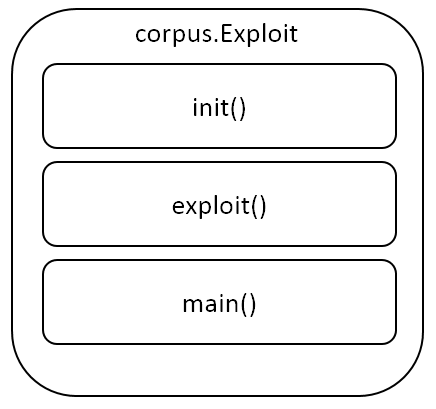
\includegraphics[scale=.5]{Corpus_Exploit.PNG}
\end{center}
\caption{Exploit Structure}
\end{figure}

\subsubsection{init()}

To annotate the exploit properly for use, we declare the name, description, references, target, type and wiki page for the exploit.  The name is the technical name specified in one of the online databases of exploits and vulnerabilities mentioned earlier in the paper.  The description is a brief statement of what the exploit is supposed to do, because the name is typically not desciptive enough for a person to understand what type of exploit is being applied.  The Target is the web application target that is being used for the exploit.  The type is the type of exploit being conducted.  The VulWikiPage is the wiki page setup for an author to place auxilliary information about the exploit or script.  The following represents an example of a XSS exploit:\\

{\tt \small

\noindent{\bf Name}:	CVE\_2012\_2403\\
{\bf Description}:		Creates a post containing a XSS payload.\\
{\bf References}:	CVE 2012-2403,OSVDB 81463 \\
{\bf Target}: 		Wordpress 3.3.1\\
{\bf Type}: 		XSS\\
{\bf VulWikiPage}: WIKIHOST/CVE-2012-2403

}

\subsubsection{exploit()}

The actual selenium script used for exploitation is contained under the exploit section.  Writing this exploit is as simple as instantiating the selenium driver and submitting a post on the wordpress site with the XSS Payload: 

{\tt \footnotesize
\begin{verbatim}

payload = "XSS PAYLOAD"

driver = self.create_selenium_driver()

driver.get("http://localhost/wordpress/?p=1")
%%Selenium Actions preceded by
% driver.find_element_by_id
("author").clear()
("author").send_keys("selenium script")
("email").clear()
("email").send_keys("selenium@python.org")
("url").clear()
("url").send_keys("www.python.org")
("comment").clear()
("comment").send_keys(payload)
("submit").click()

\end{verbatim}
}

\subsubsection{main()}

The main section handles the interface with the corpus engine, sending it the arguments parsed from the command line and the exploit function to run:

{\tt
\begin{verbatim}
    engine = corpus.Engine(Exploit())
    engine.parse_args(sys.argv)
\end{verbatim}

}


\subsection{Trace Collection}

XDebug is a feature-rich PHP extenstion which provides debugging and profiling cababilities.  For our purposes, we use it to capture traces through setting its global environment auto-trace variable.  Currently we toggle this through the command line, but want future support to be able to toggle the trace collection through the setting of cookies while the script is being executed.

\section{Scalability}
In order to create a system that can handle a growing amount of vulnerabilities that are independent from one another, we represent an exploit on an application through  Selenium scripts, as noted in the Framework section.  Selenium scripts allow us to perform operations on web applications without fear of working in an un-intended, compromised environment. 

\section{Use Cases}
By providing a corpus that explicitly logs the steps taken in accumulating the log files, we have more flexibility.  This flexibility can be seen with the following example:  
\\\\
{\tt Jon is told by his advisor that he needs to collect more trace data in order to get a proper sample size for his research.  John quickly creates a selenium script for the exploit he wants to collect and shows the advisor his results.  The advisor was generally happy with the trace data that he collected, but instead wanted him to do a slight modification to the exploit.  If Jon did not have the selenium script at hand, he would have to duplicate all of the work previously done.  Since he does have the script on hand, he can quickly make a change to the script and re-run in seconds versus hours.}
\\\\
While the above process is only shown in one iteration, most students know that this is not the case.  One hour of work can turn into a whole week of work without the proper framework in place.  The above situation also shows that the selenium script can be discussed with the professor to show validity of the data and provide talking points for how the exploit was applied.

\section{Lessons Learned}

Some research projects conducted in our software engineering group at the University of Maryland are centered around collection of metrics data for vulnerabilities.  Since we were unable to find a corpus that suited our needs, we started to build an in-house corpus.  Originally we had another VM based architecture in mind.  

\subsection{VM Architecture}
The idea was to be able to mount web application targets onto VMs.  We had a similiar idea in th sense that the VM's could be setup and brought down, saving the current state that they were in.  Once the application was mounted, we performed an exploit manually and saved a snapshot of the VM instance.  All exploits applied to "tainted" applications, so we had to be careful that one exploit did not interfere with another.  We hired summer students to create exploits and save new snapshots, from which we had them report their progress on the wiki we had built.  

\subsection{Fall Out}
We found that because the process was not documented, it was harder to verify that the exploit was executed in the correct manner.  Many times pages that were logged as exploited, did not show the representation of the exploit.  Furthermore there was no specific collection that could be analyzed of the exploit.

\subsection{Fixes}
We determined that, for one, this environment was not scalable.  We could not continue to add new exploits to a tainted environment without eventually overlapping one exploit with another.  We would have an increasingly hard time to review whether or not an exploit was overlapping.

\section{Acknowledgements}


\section{Future Development}
 \begin{description}
   \item[Distribution]
     \textcolor{red}{Virtual machine v.s. debian package. Pre-built chroot jails v.s. build scripts.
     i.e. size <--> setup proceess balance. Striking a balance between}
   \item[Services]
     \textcolor{red}{Why run Selenium/Mysql in VM vs a chroot jail?}
   \item[Isolating attack event]
     \textcolor{red}{(with xdebug manually/cookies/etc...)}   
   \item[Selenium driver and aux modules]
   Explore the possibility of a unified communication interface. This may be necessary in order to cleanly interact with xdebug with appropriate cookies set on a per-request basis (especially when modules other than Selenium are used for communication).
   \item[Payload standardization]
For each exploit currently in the corpus, there is no standard for the payload used in the attack. Since many studies may be sensitive to the payload type and encoding, it makes sense to provide the researcher with fine-grained control over this property. The Metasploit Framework has a very robust system for managing exploits along with their payloads and encodings, and can be a model for implementing this.
 \end{description}


\section{Availability}
\textcolor{red}{
[Available as a 10 GB virtual machine and as a standalone debian package?]
}
\begin{center}
{\tt git://bugbox.github.com/blahblah}
\end{center}

\begin{center}
{\tt http://www.vulnerabilitywiki.com}
\end{center}

{\footnotesize \bibliographystyle{acm}
\bibliography{ref}}

\end{document}







